\documentclass[../../main/thesis_msc.tex]{subfiles}

%% %%%%%%     README     %% %%%%%%
% addtotoc: Adds an entry to the table of contents. This option requires five
% arguments, separated by commas:
% addtotoc={page number, section, level, heading, label }
% page number : Page number of the inserted page.
% section : LATEX sectioning name – e.g., section, subsection, . . .
% level : Number, denoting depth of section – e.g., 1 for section level, 2 for
% subsection level, . . .
% heading : Title inserted in the table of contents.
% label : Name of the label. This label can be referred to with \ref and \pageref.



\begin{document}

	%\chapter{\large Type-Ia Supernovae from non-accreting progenitors}
	\chapter{Results}
	
	
	In this chapter our results are being presented in a series of two papers. In the first one, we suggest a novel progenitor channel for Supernovae-Ia along with a first-order approximation concerning the expected formation rate of the corresponding progenitor systems, energetics of the explosion, and nucleosynthetic signature. In the second one, we further explore the aforementioned progenitor channel of SNe-Ia, by creating series of stellar models with various initial values of metallicity and overshoot mixing. Finally, we elaborate on the importance of residual carbon found in ONe cores, in initiating a thermal runaway leading to the disruption of the star.
	\newline
	\noindent \textbf{Disclaimer}: What follows is an early draft version of the manuscripts submitted for publication to \textit{The Astrophysical Journal Letters}, and to \textit{The Astrophysical Journal}. Differences may appear when compared with the published version. Hence, for citing these papers please refer to the journals.
	
	\newpage
	\thispagestyle{empty}
     \null\newpage
	
		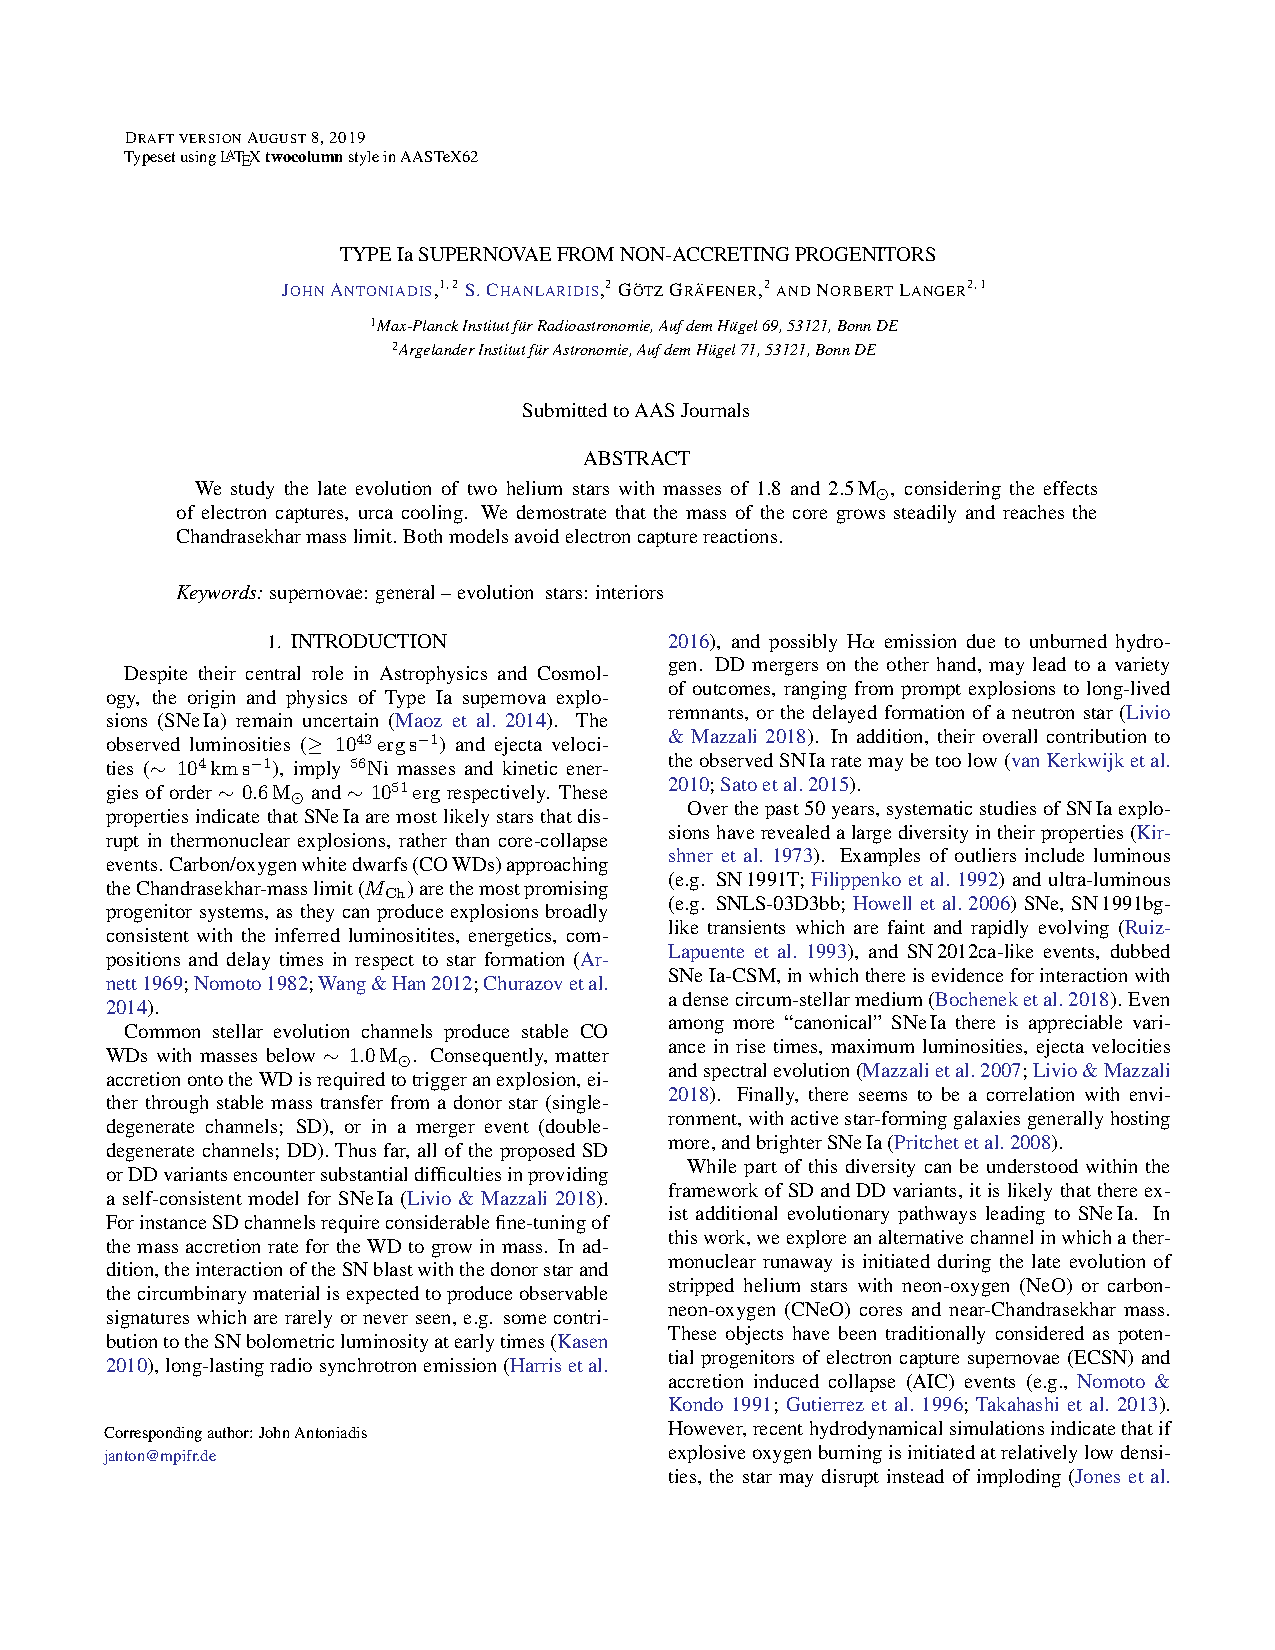
\includepdf[pages=-, scale=1.05, pagecommand={},frame=false, fitpaper=false,
            trim=0mm 0mm -10mm 0mm, addtotoc={
            1,section,1,Type-Ia supernovae from non-accreting progenitors,sec:p1,
            1,subsection,2,Introduction,p1:intro,
            2,subsection,2,(C)NeO cores: formation and evolution,p1:sec2,
            2,subsubsection,3,Numerical calculations: input physics,p1:sec2.1,
            2,subsubsection,3,Simulation results,p1:sec2.2,
            4,subsubsection,3,Late evolution and thermonuclear runaway,p1:sec2.3,
            4,subsubsection,3,Energetics and nucleosynthesis,p1:sec2.4,
            4,subsection,2,Expected rates and delay times,p1:sec3,
            6,subsection,2,Summary,p1:sec4}]{Supernovae.pdf}
            
           
            
     \thispagestyle{empty}
     \null\newpage
     
    

     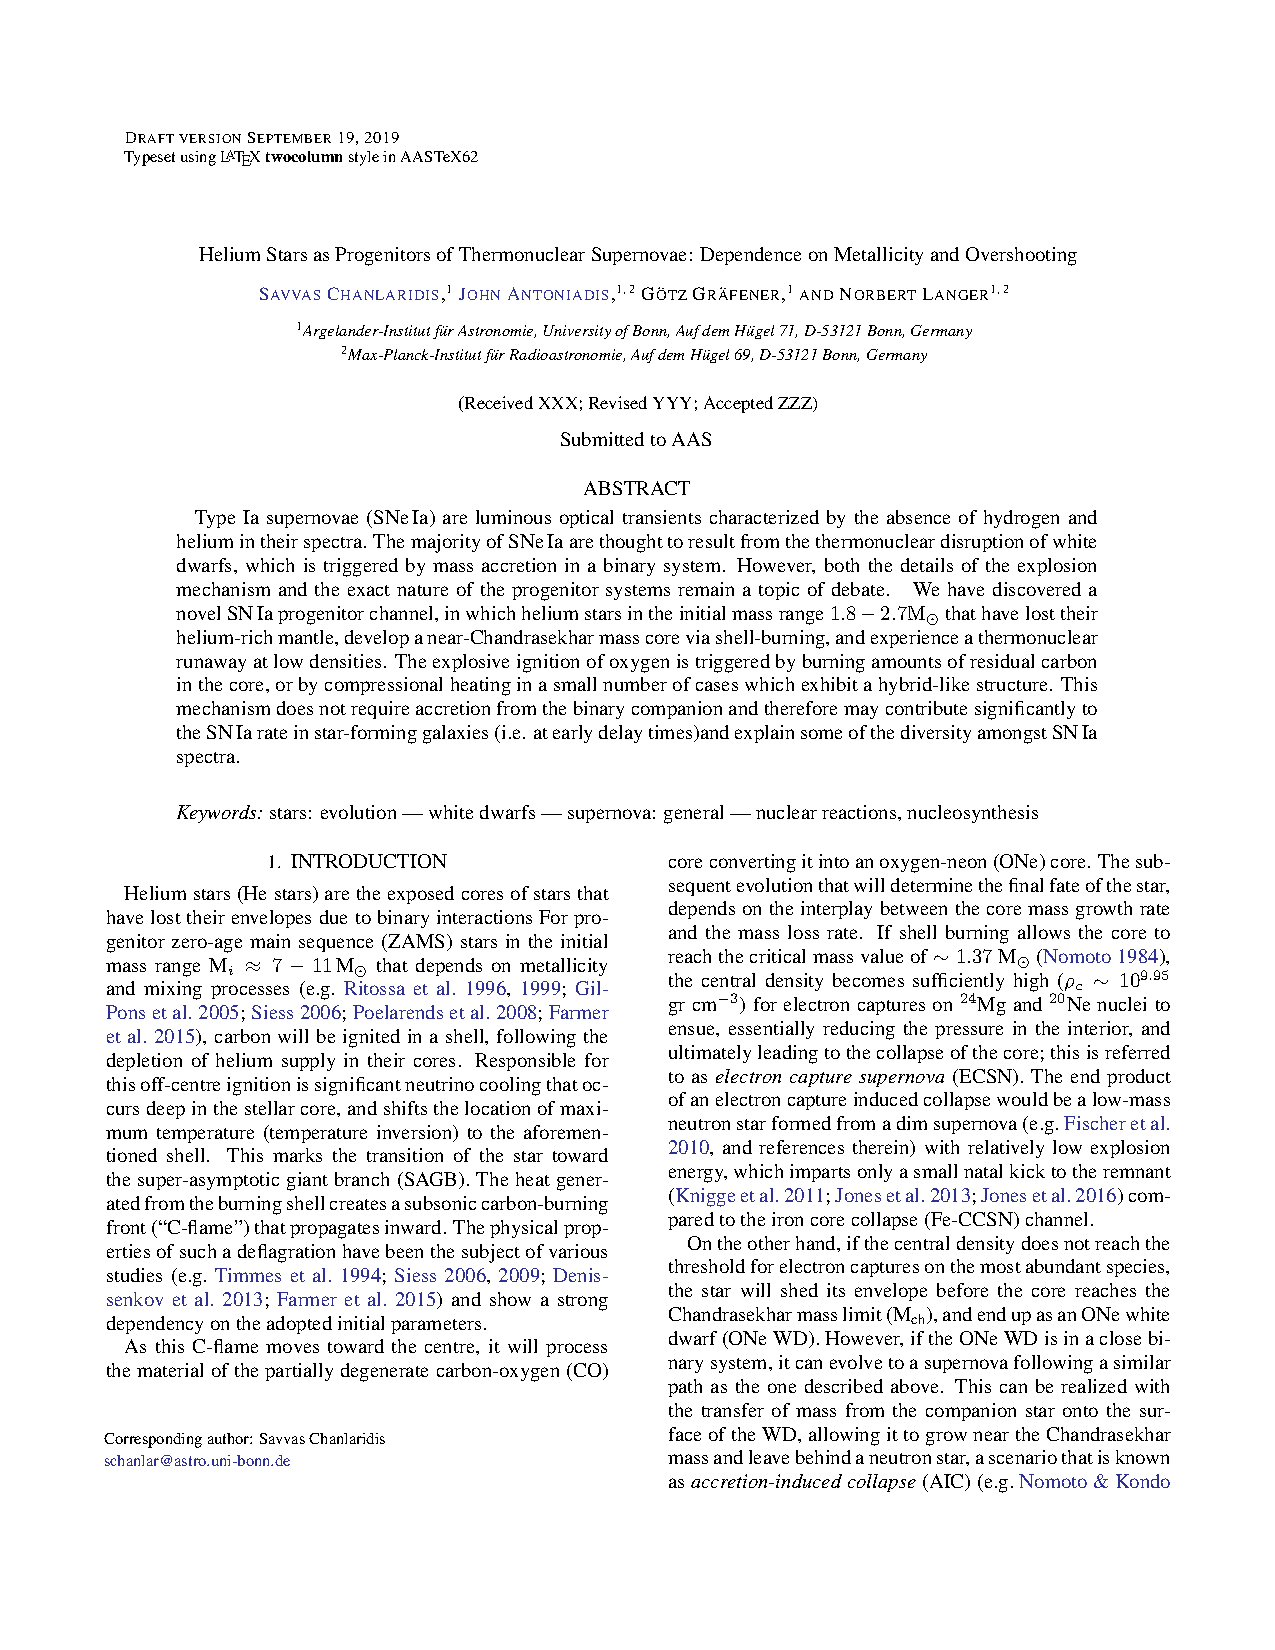
\includepdf[pages=-, scale=1.05, pagecommand={},frame=false, fitpaper=false,
            trim=0mm 0mm -10mm 0mm, addtotoc={
            1,section,1,Helium stars as progenitors of thermonuclear supernovae,sec:p2,
            1,subsection,2,Introduction,p2:intro,
            2,subsubsection,3,Thermonuclear supernovae,p2:sec1.1,
            2,subsubsection,3,The Urca process,p2:sec1.2,
            3,subsection,2,Stellar evolution code and initial parameter space,p2:sec2,
            3,subsubsection,3,Physical assumptions,p2:sec2.1,
            3,subsection,2,Results,p2:sec3,
            3,subsubsection,3,Overview of the evolution,p2:sec3.1,
            4,subsubsection,3,Core growth and structure,p2:sec3.2,
            5,subsubsection,3,Wind and ejection of inflated envelopes,p2:sec3.3,
            5,subsubsection,3,The role of residual carbon,p2:sec3.4,
            %5,subsubsubsection,4,Oxygen-Neon cores,p2:sec3.4.1,
            %5,subsubsubsection,4,Hybrid CONeMg cores,p2:sec3.4.2,
            6,subsubsection,3,Observational consequences,p2:sec3.5,
            6,subsection,2,Discussion and future work,p2:sec4}]{HeliumStars_SNeIa.pdf}
     
	

	
\end{document}